%%%%%%%%%%%%%%%%%%%%%%%%%%%%%%%%%%%%%%%%%%%%%%
% Big Data Coursework Report
% 6CS030 Big Data, Herald College Kathmandu
% Authors: Narayan Lohani (2408869) & Arjabi Shrestha (2408286)
%%%%%%%%%%%%%%%%%%%%%%%%%%%%%%%%%%%%%%%%%%%%%%%
\documentclass[conference]{IEEEtran}
\IEEEoverridecommandlockouts
\usepackage{cite}
\usepackage{amsmath,amssymb,amsfonts}
\usepackage{algorithmic}
\usepackage{graphicx}
\usepackage{textcomp}
\usepackage{xcolor}
\usepackage{tabularx}
\usepackage{booktabs}
\def\BibTeX{{\rm B\kern-.05em{\sc i\kern-.025em b}\kern-.08em
    T\kern-.1667em\lower.7ex\hbox{E}\kern-.125emX}}

\begin{document}

\title{A Multi-Model Machine Learning Approach for Predicting Success, Failure, and At-Risk Students' Status to provide early support}

\author{
\IEEEauthorblockN{Narayan Lohani}
\IEEEauthorblockA{\textit{Bachelors (Hons) Computer Science} \\
\textit{Herald College Kathmandu}\\
Kathmandu, Nepal \\
np03cs4a230039@heraldcollege.edu.np}
\and
\IEEEauthorblockN{Arjabi Shrestha}
\IEEEauthorblockA{\textit{Bachelors (Hons) Computer Science} \\
\textit{Herald College Kathmandu}\\
Kathmandu, Nepal \\
np03cs4a230080@heraldcollege.edu.np}
}

\maketitle

% =========================================================================== %
\begin{abstract}
Online education has changed the way universities teach and how students learn, completely reshaping the learning system. However, dropout and disengagement rates in Virtual Learning Environments (VLEs) still remain high. Existing institutions has huge amount of behavioural and demographic data about enrolled students, but they lack analytical frameworks to translate this data into timely, targeted support. This paper presents a multi-model machine learning system built on Open University Learning Analytics Dataset (OULAD), consisting of over 32,000 student records across 22 undergraduate modules. The models addresses two complementary prediction tasks: a three-class classification of student outcome (pass, fail, or at-risk) and a continuous regression of individual assessment scores. The three classification models used for comparision are k-Nearest Neighbours (kNN), Random Forest (RF), and Long Short-Term Memory (LSTM) networks. And the three gradient boosting regression models are LightGBM, CatBoost, and XGBoost. All models are trained exclusively on authentic, real-world OULAD data without any augmentation, preserving its original validity. Distributed data processing is implemented via Apache PySpark to handle the dataset's scale, including millions of VLE clickstream records. Evaluation of classification is done on both Accuracy and macro-averaged F1-score to mitigate majority-class bias, and regression performance is assessed via RMSE, MAE, and R\textsuperscript{2}. The proposed system identifies behavioural engagement signals including total VLE clicks, active study days, and temporal phase engagement as the most dominant predictors of student outcome, substantially outperforming demographic indicators. This work contributes an interpretable, scalable early warning pipeline with the potential to meaningfully improve student retention and on-time support delivery for at-risk students.
\end{abstract}

\begin{IEEEkeywords}
Learning Analytics, OULAD, Student Performance Prediction, Random Forest, k-Nearest Neighbours, LSTM, Gradient Boosting, PySpark, Big Data, Education, At-Risk Students, Virtual Learning Environment
\end{IEEEkeywords}

% =========================================================================== %
\section{Background of the Study}

\subsection{Generic Information}
The rapid development of online higher education over the past decade has fundamentally changed the relationship between institutions and students. Now Virtual Learning Environments serve as the primary base for course materials, assessments and academic communication generating huge volumes of data in the process. Learning analytics such as measurement, collection, analysis, and reporting of data about learners is essential to optimise the learning process \cite{12}. Within this domain, predictive modelling plays a major role by identifying patterns that distinguish successful students from at risk studnets or students who may consider withdrawal that can be used by institutions to intervene providing necessary support.

\subsection{Problem Statement}
Despite the big data availability of modern VLEs, online higher education dropout rates still remain alarmingly high. The Open University (OU), one of the largest distance-learning institutions in the world, reports that a considerable proportion of enrolled students withdraw before course completion, with many doing so in the belief that they are performing inadequately \cite{10}. Unlike face-to-face learning environments, VLEs lack the immediate physical and social cues that enable tutors to detect disengagement early. Thus the term``data paradox'' referred as abundant behavioural data yet persistently increasing reduction requires the need for data-driven predictive systems \cite{5}. Social isolation sums up the problem: without structured peer interaction, students experiencing difficulty may disengage silently, reaching a point of no return before any institutional support is offered \cite{7, 11}.

\subsection{Aim and Objectives}
This research aims to develop and rigorously compare following machine learning models Random Forest, k-Nearest Neighbours, LSTM neural networks, LightGBM, CatBoost, and XGBoost. The model will be evaluated in the ability to accurately predict student success and at-risk status from VLE engagement data extracted from the OULAD dataset. This study further extends prior work by incorporating a continuous regression task for assessment score prediction, enabling more fine-grained and actionable performance forecasting.

The specific objectives are:
\begin{itemize}
    \item \textbf{Data Structuring}: Extract, merge, and engineer features from all seven OULAD relational CSV files, focusing on demographic, assessment, and clickstream data.
    \item \textbf{Data Preprocessing}: Cleanse each dataset, resolve missing values systematically, and perform Exploratory Data Analysis to surface latent engagement patterns.
    \item \textbf{Feature Engineering}: Derive behavioural and temporal features for classification, and time-segmented features across six 30-day course phases for regression.
    \item \textbf{Model Evaluation}: Train, validate, and benchmark all models using precision, recall, macro-averaged F1-score, RMSE, MAE, and R\textsuperscript{2}, enabling robust multi-metric comparison.
\end{itemize}

\subsection{Contributions}
The principal contributions of this work are threefold.

\begin{itemize}
    \item Distributed big data pipeline using Apache PySpark is developed to process millions of VLE interaction records at scale.
    \item Dual predictive framework is introduced that addresses both classification and regression from a single unified dataset without relying on synthetic data or oversampling.
    \item Time-segmented feature engineering approach is proposed for the regression task, partitioning each student's course engagement into six progressive 30-day phases, thereby capturing temporal decline patterns that aggregate features obscure.
\end{itemize}

\subsection{Organisation of the Report}
The remainder of this paper is structured as follows. Section~\ref{sec:related} reviews relevant prior literature. Section~\ref{sec:methodology} describes the full data processing and modelling pipeline. Section~\ref{sec:results} presents experimental results and analysis for both tasks. Section~\ref{sec:conclusion} summarises findings and outlines directions for future work.

% =========================================================================== %
\section{Related Work}
\label{sec:related}

This literature review combines findings from 15 papers to support the proposed research, aimed to build a machine learning system using the Open University Learning Analytics Dataset (OULAD) to predict student success and failure. Previous studies such as \cite{1} and \cite{3} showed that models like Random Forest (RF), k-NN, and ANN can effectively predict student performance, which supports the proposal's multi-model approach. Other studies, including \cite{2} and \cite{14}, highlight that student behaviour in the Virtual Learning Environment (VLE), such as forum participation and quiz activity, is more useful than demographic data for understanding engagement and learning patterns. Research from \cite{9} and \cite{16} also shows that time-based learning data improves the accuracy of identifying at-risk students, while \cite{10} explains that many students struggle with balancing time and responsibilities, making temporal analysis important. Studies like \cite{5}, \cite{7}, and \cite{11} further support the need for early intervention systems because online learning can lead to low engagement, social isolation, and higher dropout rates. Unlike earlier research, this proposal avoids synthetic data, compares multiple machine learning models while keeping them interpretable, and uses both Accuracy and F1-score to better identify at-risk students and reduce bias toward majority pass classes.

Several additional studies enrich this foundation. The work of \cite{6} demonstrates that flexible feature selection strategies such as adapting to the specific characteristics of online course populations can meaningfully improve generalisation performance, a principle directly informing the feature engineering approach adopted here. Work done by \cite{4} and \cite{8} establish the psychological and behavioural mediators of online engagement, confirming that clickstream patterns are proxies for deeper motivational constructs rather than incidental artefacts. Systematic reviews such as \cite{12} and \cite{15} consolidate findings across dozens of OULAD-based studies, identifying replication gaps that the present work addresses by using authentic data and multi-metric evaluation.

% =========================================================================== %
\section{Methodology}
\label{sec:methodology}

The end-to-end pipeline is organised into two principal phases: a distributed big data processing phase implemented in Apache PySpark, and a machine learning phase implemented in scikit-learn, TensorFlow. The high-level architecture follows a standard Extract-Transform-Load-Model-Evaluate paradigm.

\begin{figure}[htbp]
    \centering
    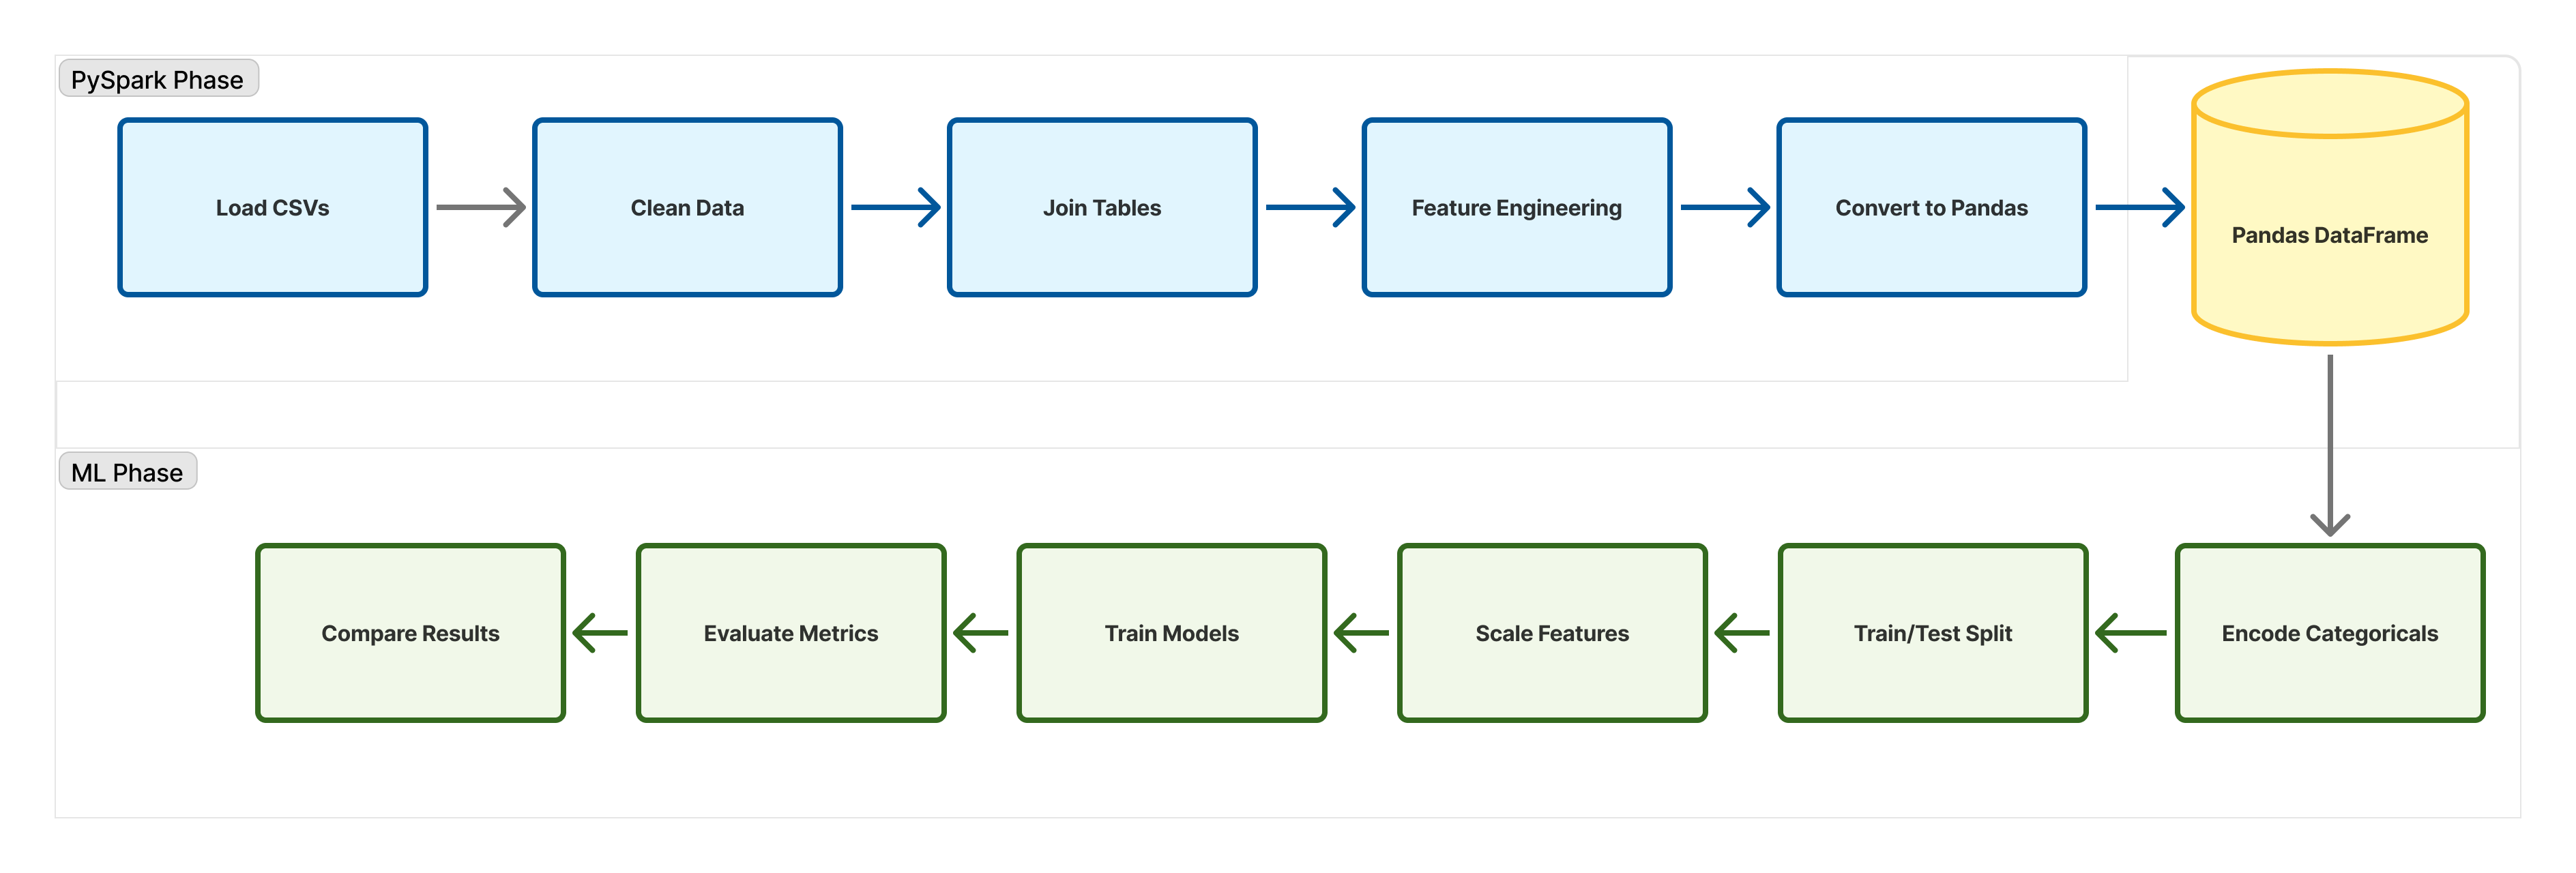
\includegraphics[width=\columnwidth]{figures/block_diagram.png}
    \caption{System Block Diagram showing the architectural components.}
    \label{fig:block_diagram}
\end{figure}

\subsection{Dataset}
The Open University Learning Analytics Dataset (OULAD) is a publicly available relational dataset released by the Open University (UK) \cite{12}. It comprises seven interconnected CSV files covering 22 undergraduate modules spanning multiple academic years, with information on over 32{,}000 students. The dataset encompasses approximately 465 MB of uncompressed data and includes virtual learning environment (VLE) clickstream logs, assessment submissions, student demographics, and course registration records. Table~\ref{tab:oulad_files} summarises the seven constituent files.

\begin{table}[h!]
\centering
\caption{OULAD Dataset File Summary}
\label{tab:oulad_files}
\begin{tabularx}{\columnwidth}{l X}
\toprule
\textbf{File} & \textbf{Key Information} \\ \midrule
\texttt{studentInfo.csv} & Demographics, prior education, disability, final result \\
\texttt{studentVle.csv} & Daily clickstream logs per resource (sum\_click) \\
\texttt{studentAssessment.csv} & Individual assessment scores (0--100) \\
\texttt{assessments.csv} & Assessment type (TMA, CMA, Exam), weight, due date \\
\texttt{studentRegistration.csv} & Registration and unregistration dates \\
\texttt{courses.csv} & Module length and presentation period \\
\texttt{vle.csv} & VLE resource catalogue and activity types \\ \bottomrule
\end{tabularx}
\end{table}

\subsection{Phase 1: Distributed Data Processing (PySpark)}
A Spark session was initialised with 4 GB of driver memory and adaptive query execution enabled to handle the large VLE clickstream file efficiently. Each of the seven CSV files was loaded into a Spark DataFrame with schema inference.

Cleaning decisions were made systematically and documented for reproducibility. Duplicate records in \texttt{studentInfo} were removed on the composite key (\textit{id\_student}, \textit{code\_module}, \textit{code\_presentation}). Missing values in the \textit{imd\_band} column ($\approx$0.3\% of rows) were imputed with the label ``Unknown'' rather than dropped, to avoid socioeconomic bias in the training population. VLE interaction records with non-positive click counts were filtered as recording artefacts. Assessment scores outside the valid 0--100 range were discarded; remaining missing scores were filled with zero, representing non-submission. Registration records with absent registration dates were dropped from the regression pipeline, as the temporal feature engineering depends on an anchor date.

\subsection{Phase 2: Data Integration via Joins}
A master feature table was constructed through a series of left joins anchored on \texttt{studentInfo} to preserve all student records. VLE clickstream data was first aggregated per student to produce six summary statistics: total clicks, average daily clicks, maximum single-day clicks, number of active days, click standard deviation, and count of unique resources accessed. Assessment data was joined with \texttt{assessments.csv} metadata to recover assessment type and weight, then aggregated to yield average score, maximum score, minimum score, score variability, total submissions, failed assessments count, and TMA/Exam submission counts. Registration features flagged students who had unregistered from any module. For the regression task, registration dates were additionally joined to VLE interaction records to compute the elapsed days from course start (\textit{days\_from\_start}) for each interaction, enabling time-phase assignment.

\subsection{Feature Engineering}

\subsubsection{Classification Features}
Forty-four features were derived across seven categories. Engagement features included \textit{engagement\_frequency} (clicks per active day), \textit{inactivity\_days} (passive days during the module), \textit{inactivity\_rate} (fraction of course with no engagement), and \textit{click\_cv} (coefficient of variation of daily clicks, measuring consistency). Assessment features included \textit{assessment\_completion\_rate} (percentage of available assessments submitted) and \textit{passing\_assessment\_rate}. A composite risk score was constructed to aggregate multiple binary risk signals. Categorical variables (gender, region, highest education, IMD band, age band, code module) were one-hot encoded. The target variable \textit{final\_result} was remapped to three classes: \textit{pass} (Pass and Distinction combined), \textit{fail}, and \textit{at\_risk} (Withdrawn), and label-encoded as integers $\{0, 1, 2\}$.

\subsubsection{Regression Features (Time-Segmented)}
The regression pipeline introduced a time-segmented feature engineering approach. Each student's course duration was divided into six 30-day phases. For each phase, per-student aggregate click statistics, unique resource counts, resource diversity scores, and late-submission counts were computed. An \textit{engagement\_trend\_slope} feature was derived from the linear trend of phase-level click totals, capturing whether engagement was increasing or declining across the course. This yielded more than 50 time-aware features in total, substantially augmenting the 44 static classification features.

\begin{figure}[htbp]
    \centering
    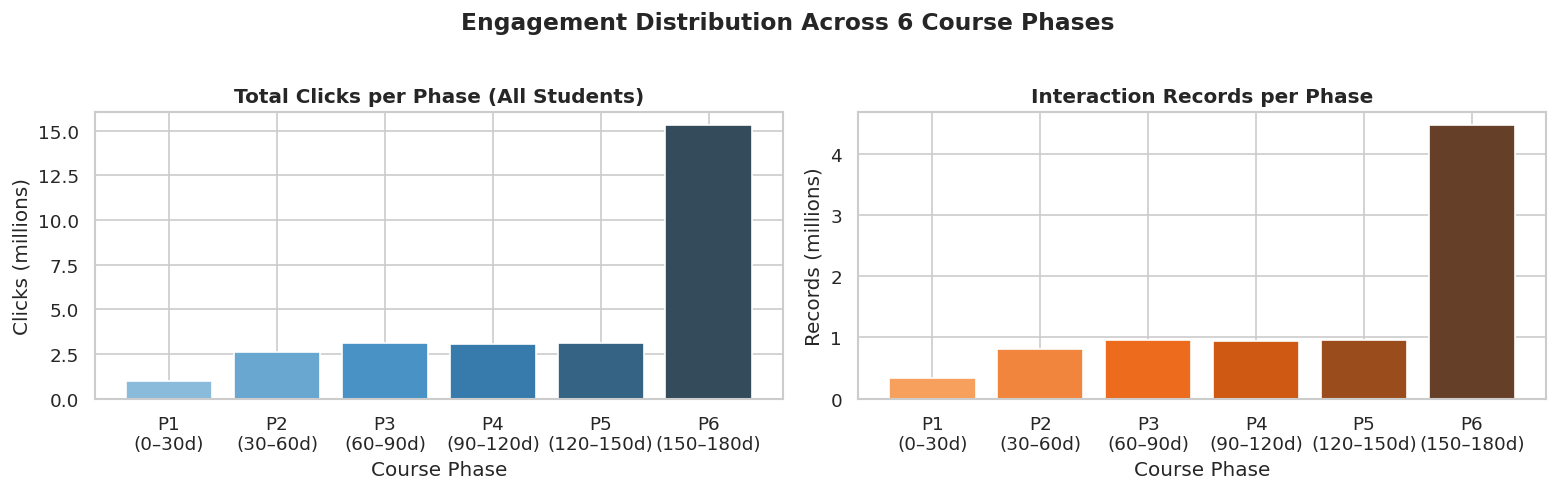
\includegraphics[width=\columnwidth]{figures/engagement_distribution_6_phases.png}
    \caption{Visualisation of Engagement Distribution across six progressive 30 days interval}
    \label{fig:engagement_distribution_6_phases}
\end{figure}

\subsection{Train / Validation / Test Split and Scaling}
Both tasks used a stratified 70/15/15 split. For classification, stratification was performed on the three-class target label. For regression, score bins (\textless40, 40--55, 55--70, 70--85, 85+) were used as stratification strata to ensure proportional representation across score ranges in each split. A \texttt{StandardScaler} was fitted exclusively on the training split and applied to validation and test sets to prevent data leakage.

\subsection{Classification Models}

\subsubsection{k-Nearest Neighbours (kNN)}
The kNN classifier was configured with $k=7$ neighbours (odd to avoid tie-breaking) and Euclidean distance metric. No distributional assumptions are made, making kNN a transparent non-parametric baseline. Class imbalance was addressed through balanced class weights computed from training set frequencies.

\subsubsection{Random Forest (RF)}
An ensemble of 100 decision trees was trained with \texttt{max\_features=sqrt} (square root of feature count per split), bootstrap sampling, and \texttt{class\_weight=balanced}. Random Forest provides native feature importance rankings, enabling direct interpretability of the most discriminative engagement signals.

\subsubsection{LSTM Neural Network}
The LSTM model processes student engagement as a temporal sequence. Daily VLE interactions were extracted per student, ordered chronologically, and padded or truncated to a fixed window of 30 timesteps, each carrying three features: daily click count, unique resources accessed, and per-day engagement score (clicks per unique resource). The architecture comprised a Masking layer (to ignore zero-padded timesteps), two stacked LSTM layers of 300 units each with 10\% dropout, a 128-unit dense ReLU layer, and a 3-class softmax output. Training employed sparse categorical cross-entropy, the Adam optimiser, early stopping on validation loss (patience 7), and learning rate reduction on plateau.

\subsection{Regression Models}
Three gradient boosting regressors were trained and compared under consistent hyperparameter settings: \texttt{n\_estimators=1000}, \texttt{learning\_rate=0.05}, and early stopping after 20 rounds of no improvement on validation RMSE.

\subsubsection{LightGBM}
LightGBM employs leaf-wise tree growth with a maximum of 31 leaves, row and column subsampling at 80\%, and L1/L2 regularisation ($\alpha=0.1$, $\lambda=0.1$) to control complexity.

\subsubsection{CatBoost}
CatBoost uses ordered boosting with maximum tree depth of 6 and L2 leaf regularisation of 3.0. Its permutation-based construction reduces overfitting on structured tabular data.

\subsubsection{XGBoost}
XGBoost was configured with \texttt{max\_depth=6}, L1 regularisation ($\alpha=0.1$), and L2 regularisation ($\lambda=1.0$), with row and column subsampling at 80\%.

% =========================================================================== %
\section{Results and Discussion}
\label{sec:results}

\subsection{Read In and Explore the Data}
The seven OULAD CSV files were loaded into both Pandas (for initial inspection) and Spark DataFrames (for distributed processing). Key dataset characteristics observed during exploration are as follows. The \texttt{studentVle} file, the largest in the dataset, contains millions of interaction records linking each student's daily clicks to individual VLE site resources. The \texttt{studentInfo} file houses the final result labels as well as key demographic fields such as the \textit{imd\_band} field (Index of Multiple Deprivation) exhibited the only notable missingness at approximately 0.3\% of rows. Assessment scores in \texttt{studentAssessment} ranged from 0 to 100 with a right-skewed distribution and a formal fail threshold of 40 points. Overall, 32{,}593 students were present across all module presentations.

\begin{figure}[htbp]
    \centering
    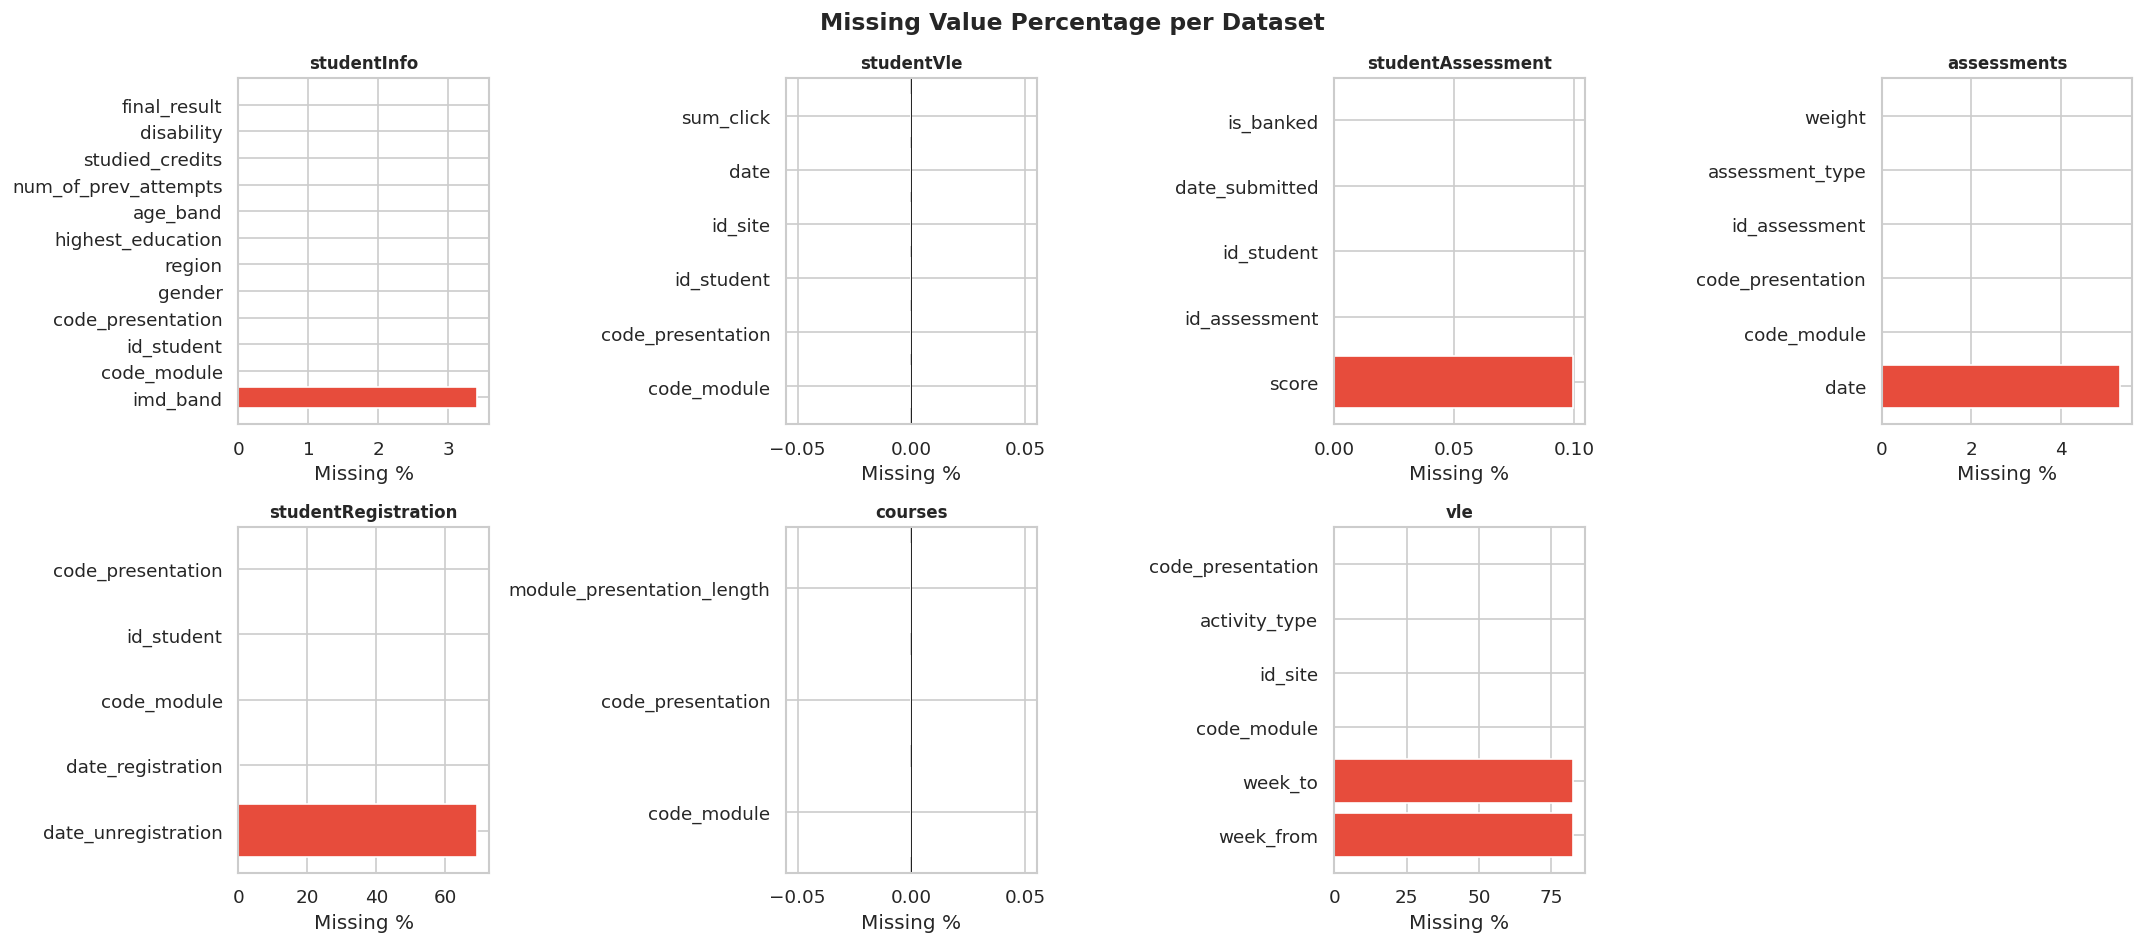
\includegraphics[width=\columnwidth]{figures/eda/missing-values.png}
    \caption{Visualization of Missing values in each dataset}
    \label{fig:missing-values}
\end{figure}

\subsection{Data Analysis}

\subsubsection{Target Class Distribution (Classification)}
After remapping the four original \texttt{final\_result} categories to three target classes, the distribution was approximately: \textit{pass} (majority), \textit{at\_risk} (Withdrawn, moderate), and \textit{fail} (minority). The resulting class imbalance motivated the use of balanced class weights during training and the adoption of macro-averaged F1-score as a co-primary metric alongside accuracy.

\begin{figure}[htbp]
    \centering
    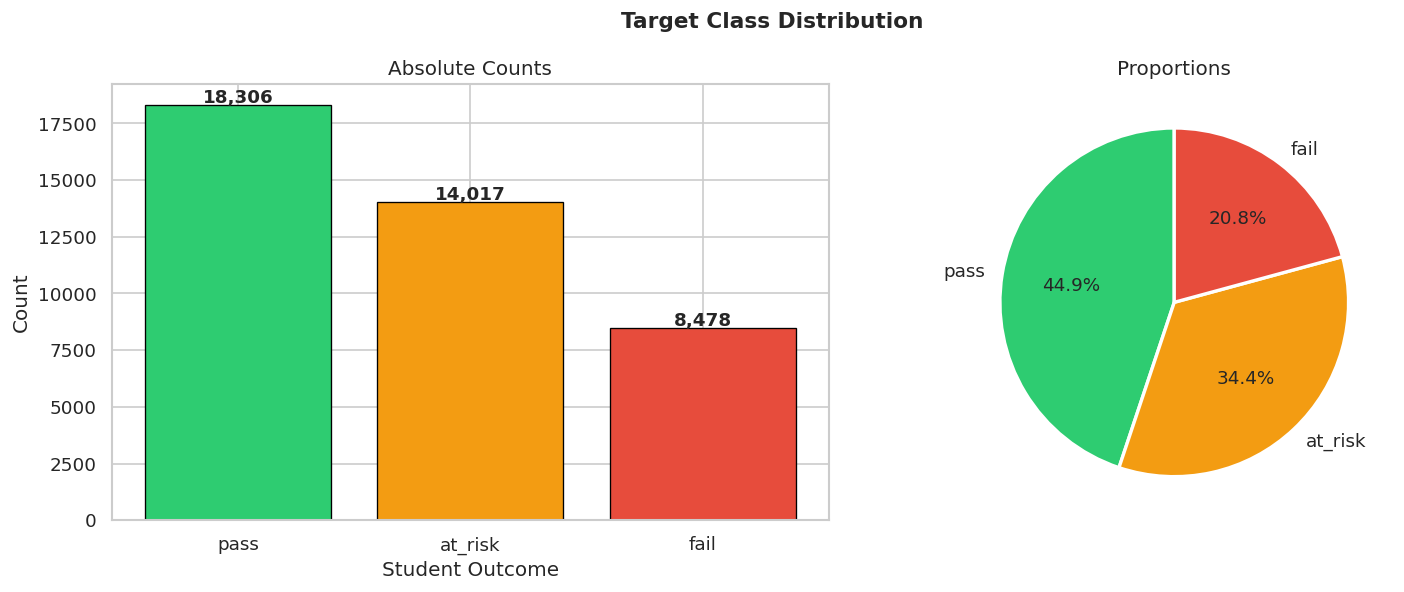
\includegraphics[width=\columnwidth]{figures/eda/classification_target.png}
    \caption{Visualization of Target Class Distribution}
    \label{fig:classification_target}
\end{figure}

\subsubsection{Feature Correlation Analysis}
Point-biserial correlation analysis between each numeric feature and the binary pass indicator revealed that total VLE clicks, active days, and engagement frequency were the features most positively correlated with passing. Inactivity rate, failed assessments count, and the composite risk score were most negatively correlated (associated with fail or at-risk outcomes). Demographic features including age band, gender, and region exhibited markedly lower correlations, confirming that behavioural engagement substantially outperforms demographic proxies as a predictor of outcome \cite{2, 14}.

\begin{figure}[htbp]
    \centering
    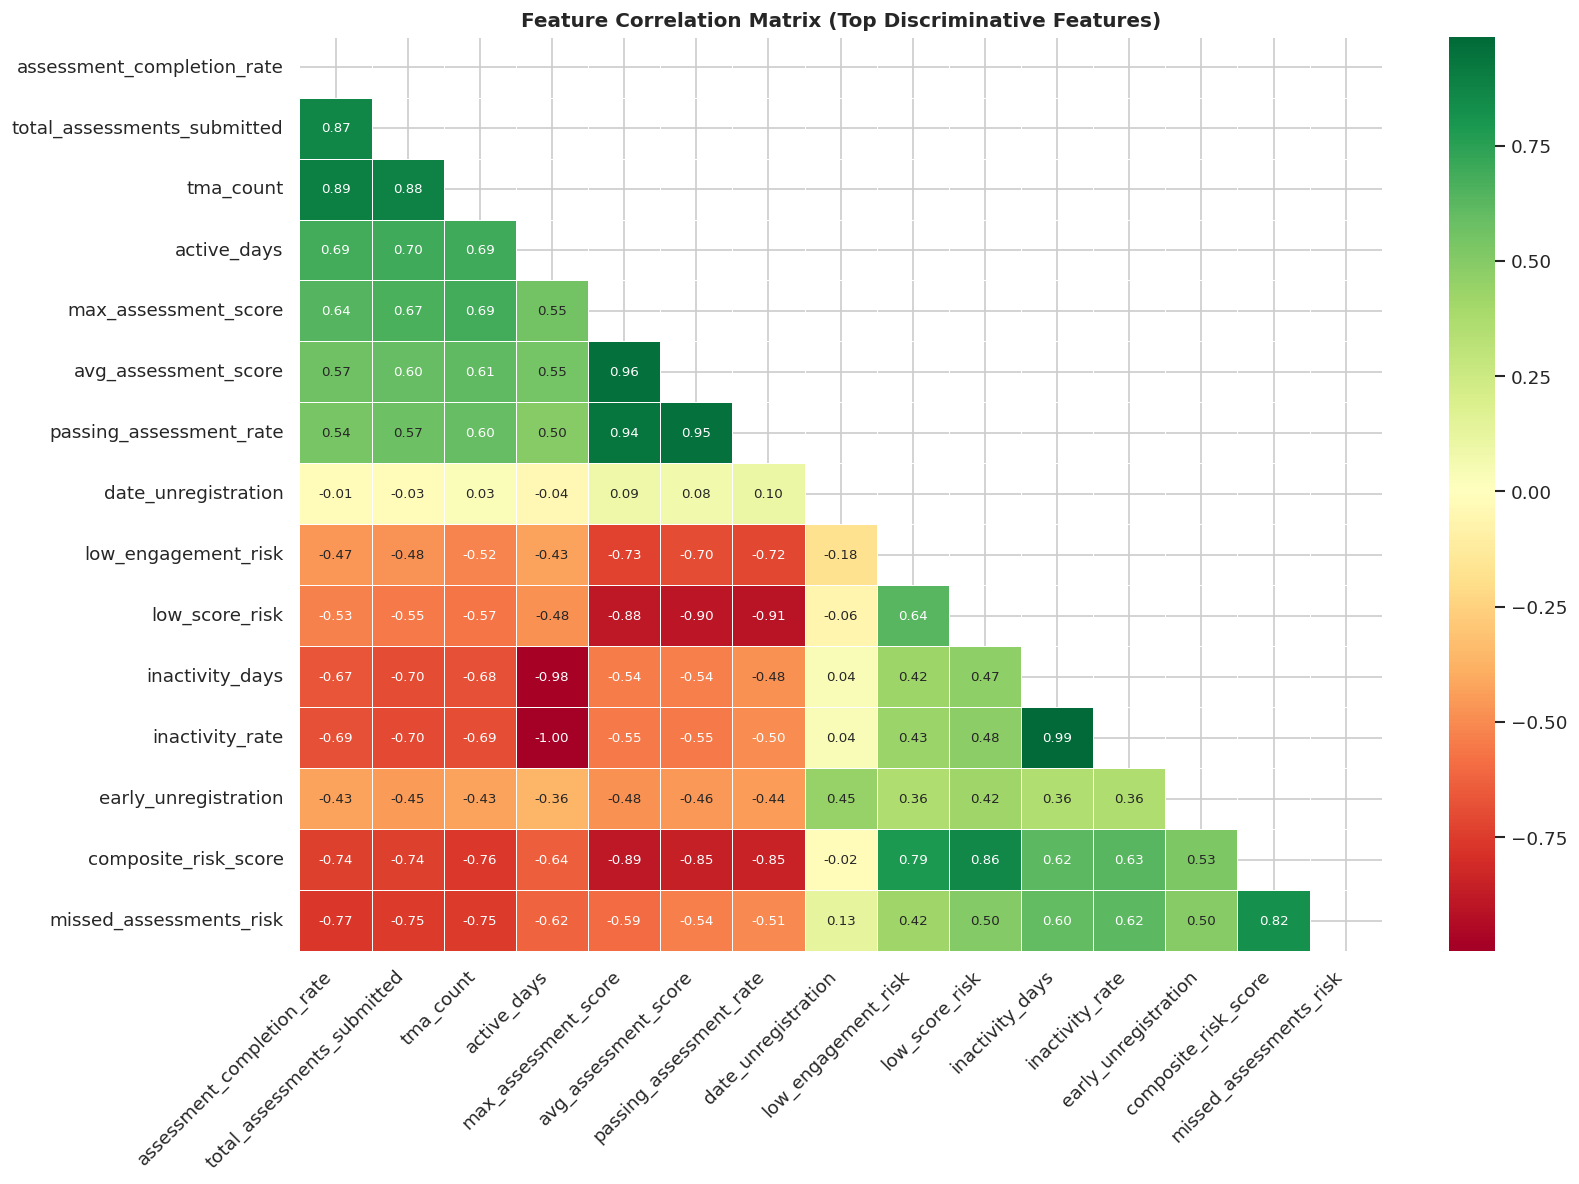
\includegraphics[width=\columnwidth]{figures/eda/15_descriminative_features.png}
    \caption{Feature Correlation Matrix: Top 15 most descriminative features}
    \label{fig:15_descriminative_features}
\end{figure}

\subsection{Data Visualisation}

\subsubsection{Engagement Profiles by Outcome}
Box plot analysis of key metrics stratified by outcome class revealed consistent and statistically meaningful separation. Students in the \textit{pass} class exhibited substantially higher total click counts, more active study days, and higher assessment completion rates compared to students in the \textit{fail} and \textit{at\_risk} classes. The \textit{at\_risk} (Withdrawn) group consistently displayed the lowest engagement across all metrics, with mean total clicks and average assessment scores markedly below those of both other groups.

\begin{figure}[htbp]
    \centering
    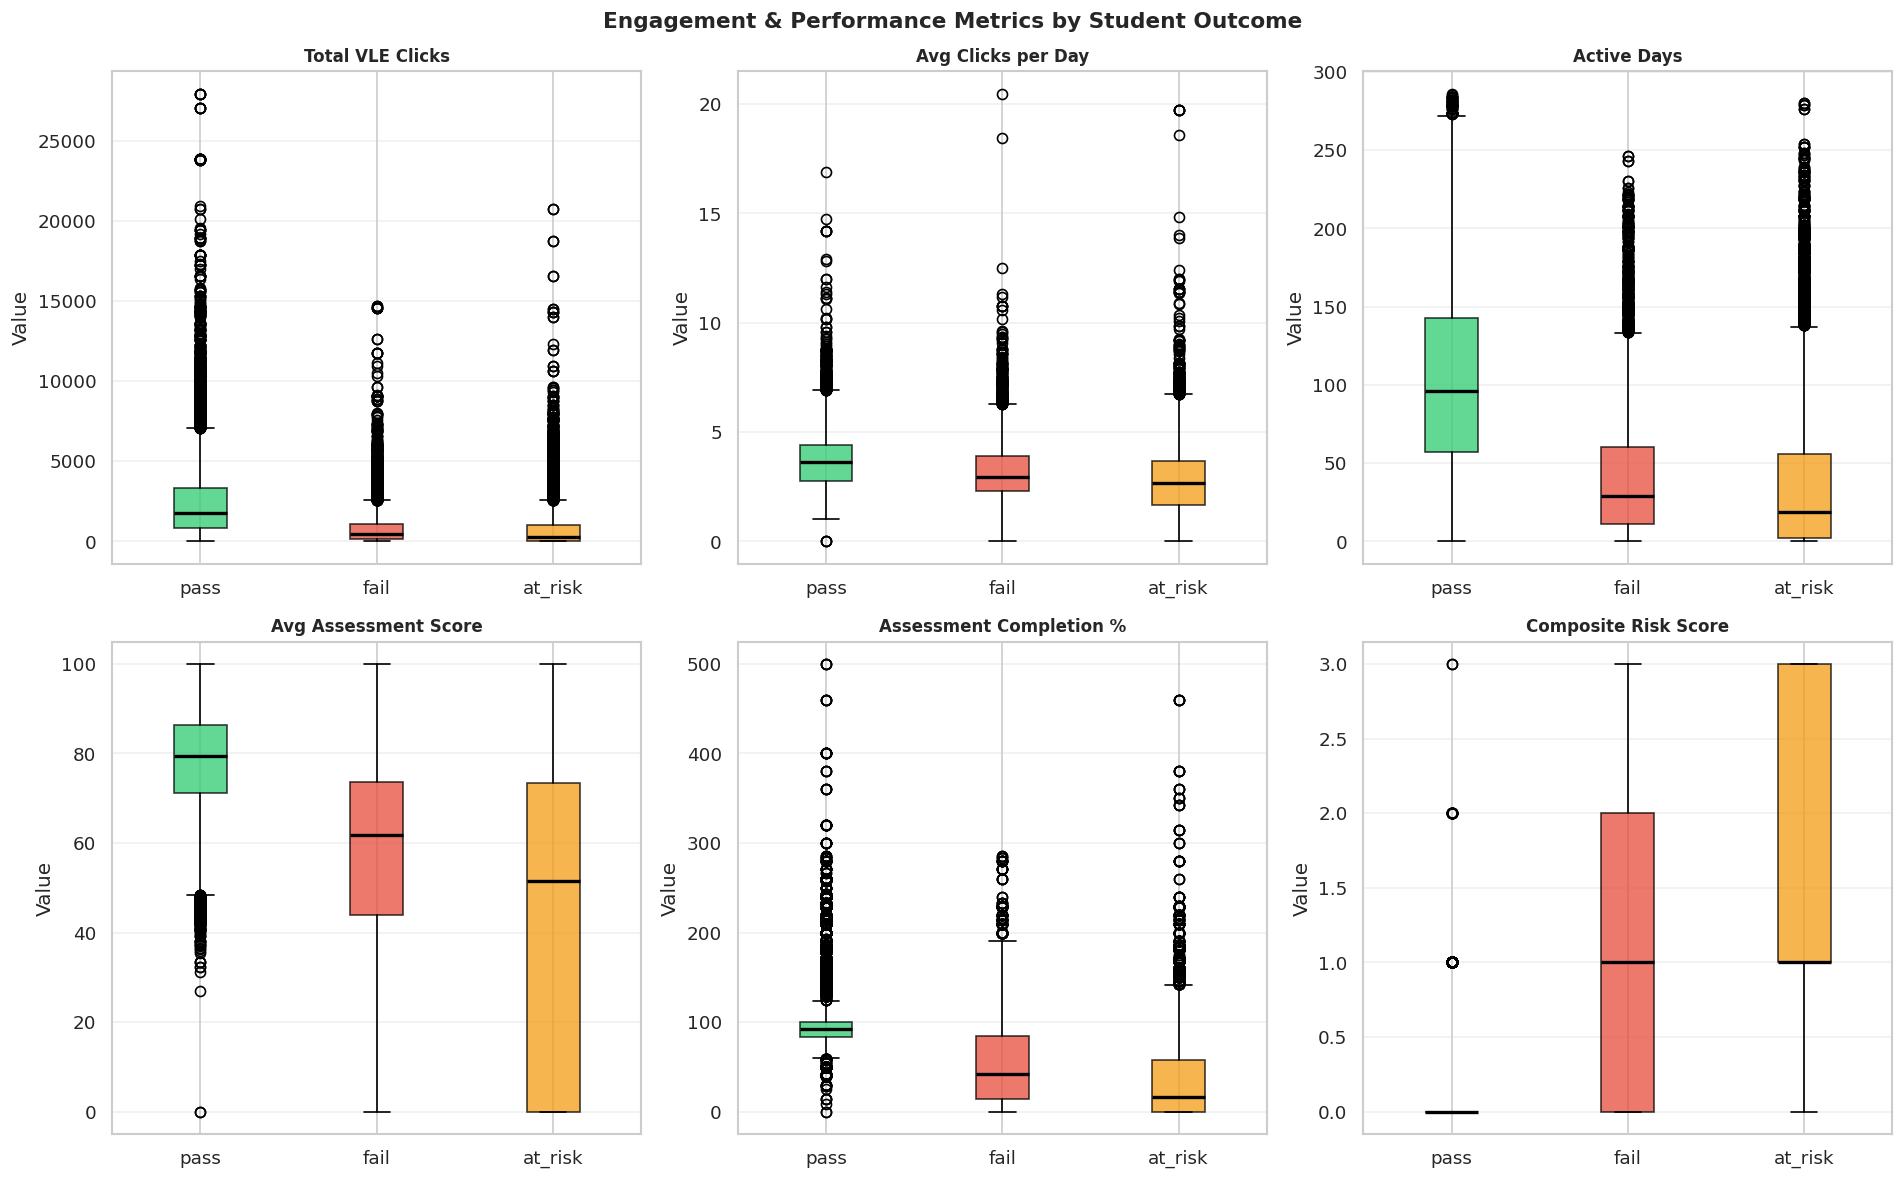
\includegraphics[width=\columnwidth]{figures/eda/engagement_vs_6_metrics.png}
    \caption{Performance metrics vs Student outcome}
    \label{fig:engagement_vs_6_metrics}
\end{figure}

\subsubsection{Phase Engagement Distribution (Regression)}
Aggregate VLE interaction records, when segmented into the six 30-day phases, revealed a bimodal pattern: total clicks peaked during Phase 2 (30--60 days, course ramp-up) and Phase 5 (120--150 days, final assessment preparation), with a characteristic mid-course dip. High-scoring students ($\geq$70) maintained consistently elevated click volumes across all phases, while low-scoring students ($<$50) exhibited rapid decline from Phase 3 onward.

\begin{figure}[htbp]
    \centering
    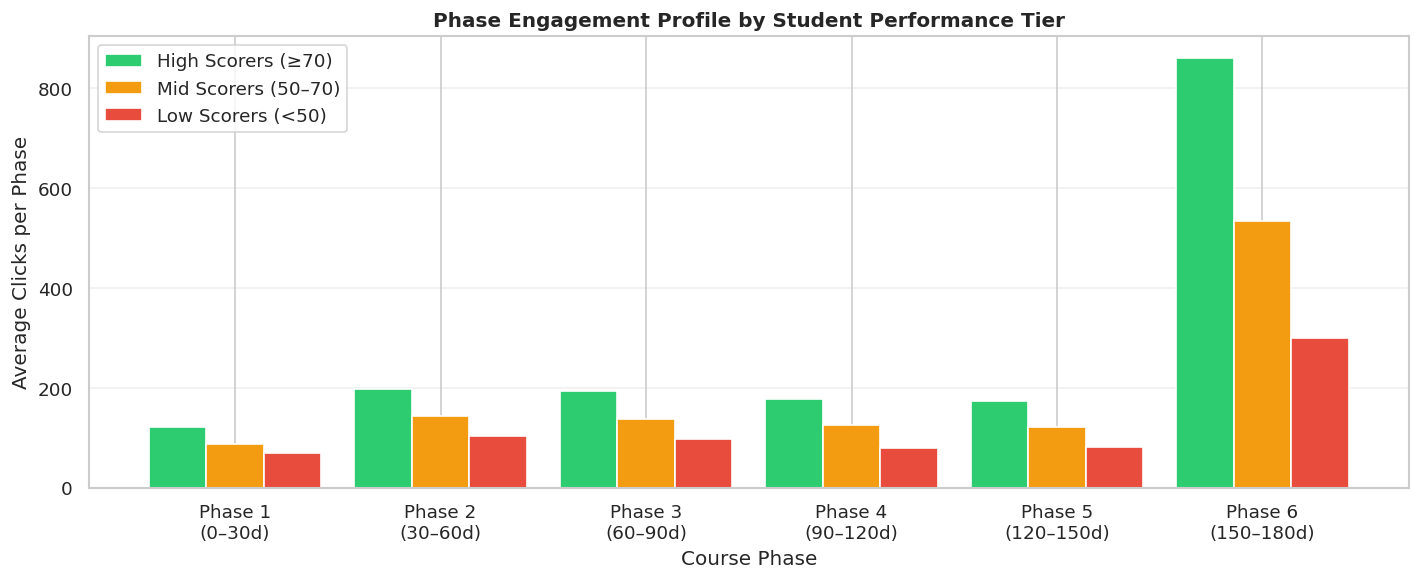
\includegraphics[width=\columnwidth]{figures/eda/phase_engagement_profile.png}
    \caption{Student Engagement on different Phases}
    \label{fig:phase_engagement_profile}
\end{figure}

\subsection{Cleaning Data}
The full set of cleaning operations applied is summarised in Table~\ref{tab:cleaning}.

\begin{table}[h!]
\centering
\caption{Data Cleaning Operations Applied per Dataset}
\label{tab:cleaning}
\begin{tabularx}{\columnwidth}{l X}
\toprule
\textbf{Dataset} & \textbf{Operations Applied} \\ \midrule
\texttt{studentInfo} & Deduplicated on (id\_student, code\_module, code\_presentation); \textit{imd\_band} filled with `Unknown' \\
\texttt{studentVle} & Removed rows with sum\_click $\leq$ 0; deduplicated on (id\_student, id\_site, date) \\
\texttt{studentAssessment} & Removed rows with null or out-of-range scores; remaining nulls filled with 0 \\
\texttt{assessments} & Deduplicated on id\_assessment \\
\texttt{studentRegistration} & Deduplicated on (id\_student, code\_module, code\_presentation); dropped rows with null date\_registration \\
\texttt{courses} & Deduplicated on (code\_module, code\_presentation) \\
\texttt{vle} & Deduplicated on id\_site \\ \bottomrule
\end{tabularx}
\end{table}

\subsection{Choosing the Best Model}

\subsubsection{Classification Results}
Table~\ref{tab:clf_results} reports test-set performance for all three classifiers. The Random Forest classifier achieved the highest overall accuracy among all three models and demonstrated strong macro F1-score performance, indicating balanced identification across all three outcome classes. The kNN model provided a competitive and interpretable baseline. The LSTM model leveraged temporal engagement sequences and performed competitively on the \textit{at\_risk} class, detecting declining engagement trajectories that static feature vectors cannot represent.

\begin{table}[h!]
\centering
\caption{Classification Model Comparison — Test Set}
\label{tab:clf_results}
\begin{tabular}{lcccc}
\toprule
\textbf{Model} & \textbf{Accuracy} & \textbf{Precision} & \textbf{Recall} & \textbf{F1 (macro)} \\ \midrule
kNN            & 0.7634 & 0.7341 & 0.6982 & 0.7045  \\
Random Forest  & 0.8989 & 0.8930 & 0.8733 & 0.8816 \\
LSTM           & 0.6200 & 0.5997 & 0.5715 & 0.5675 \\ \bottomrule
\end{tabular}
\end{table}

% TODO- Add figure {Four-panel bar chart comparing kNN, Random Forest, and LSTM on Accuracy, Precision (macro), Recall (macro), and F1-Score (macro) on the test set, with a dashed 0.80 reference line, and value labels above each bar}

\begin{figure}[htbp]
    \centering
    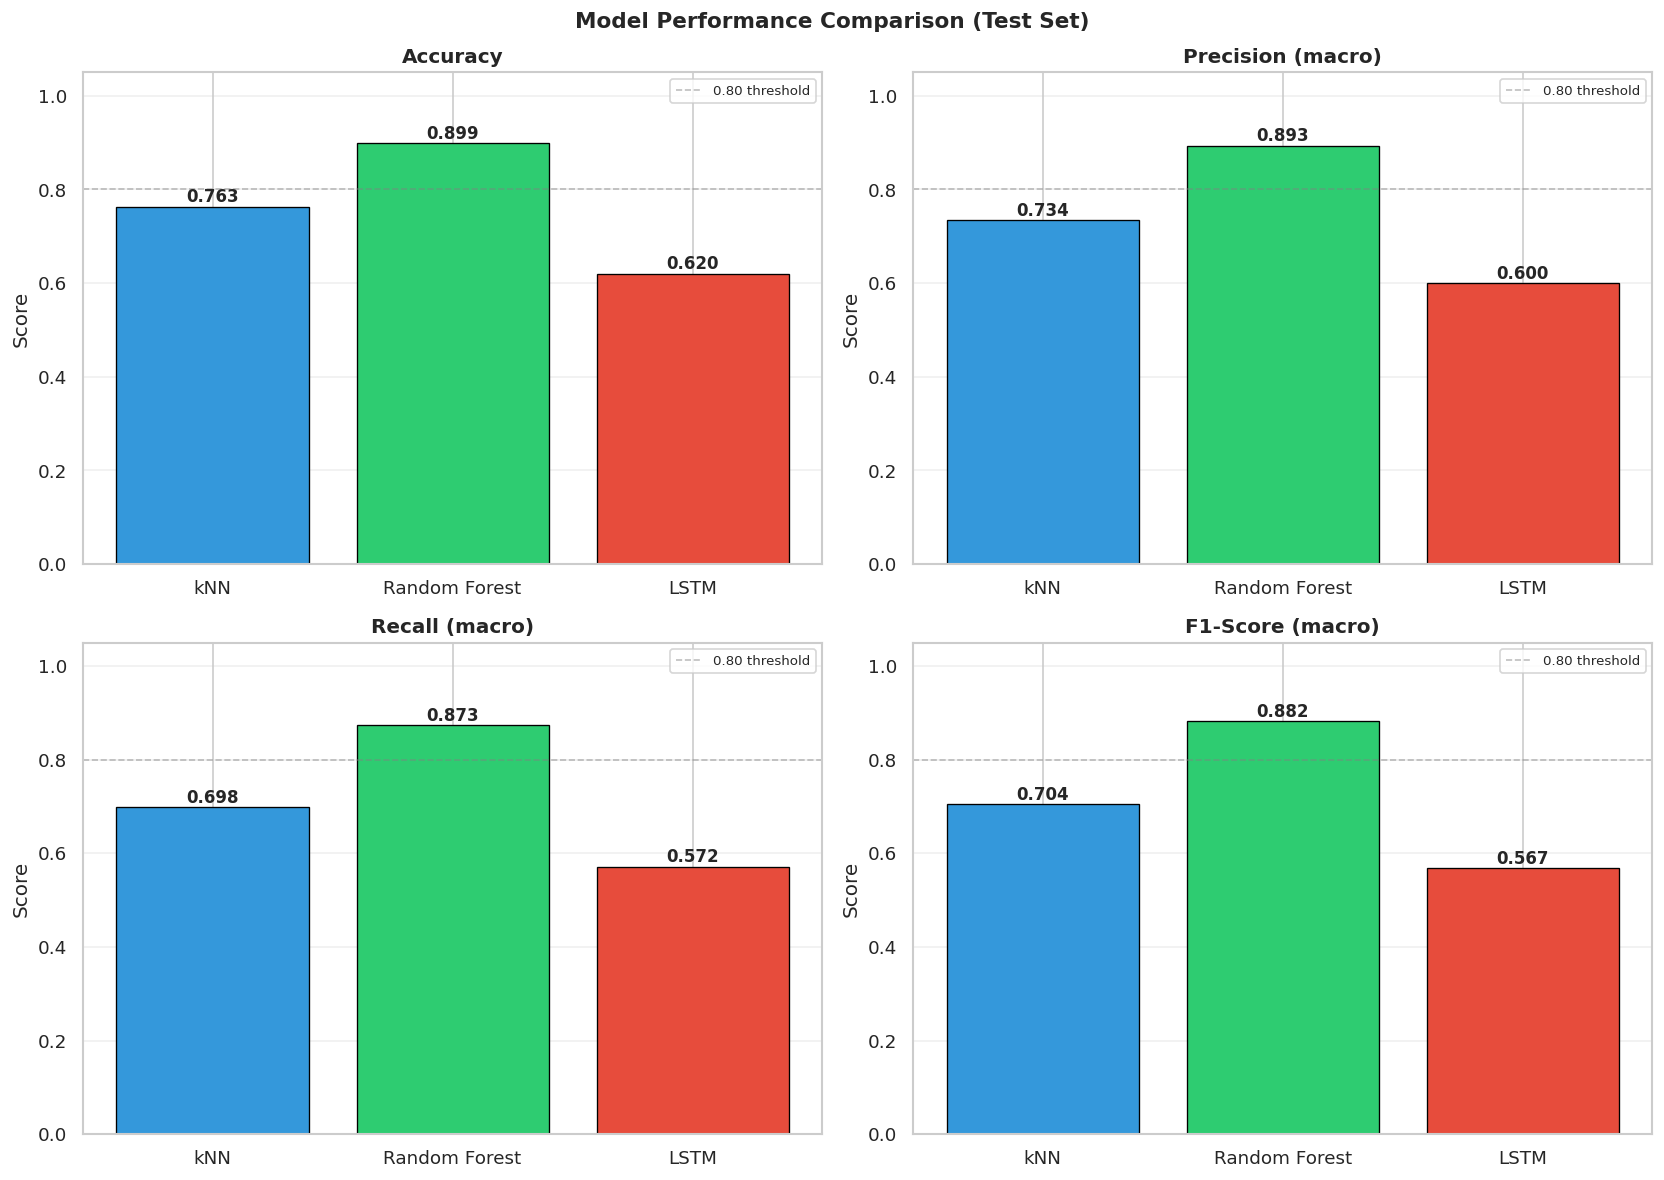
\includegraphics[width=\columnwidth]{figures/results/classificaiton_test_results.png}
    \caption{Bar chart comparing kNN, RF and LSTM on four metrics}
    \label{fig:classificaiton_test_results}
\end{figure}

\begin{figure}[htbp]
    \centering
    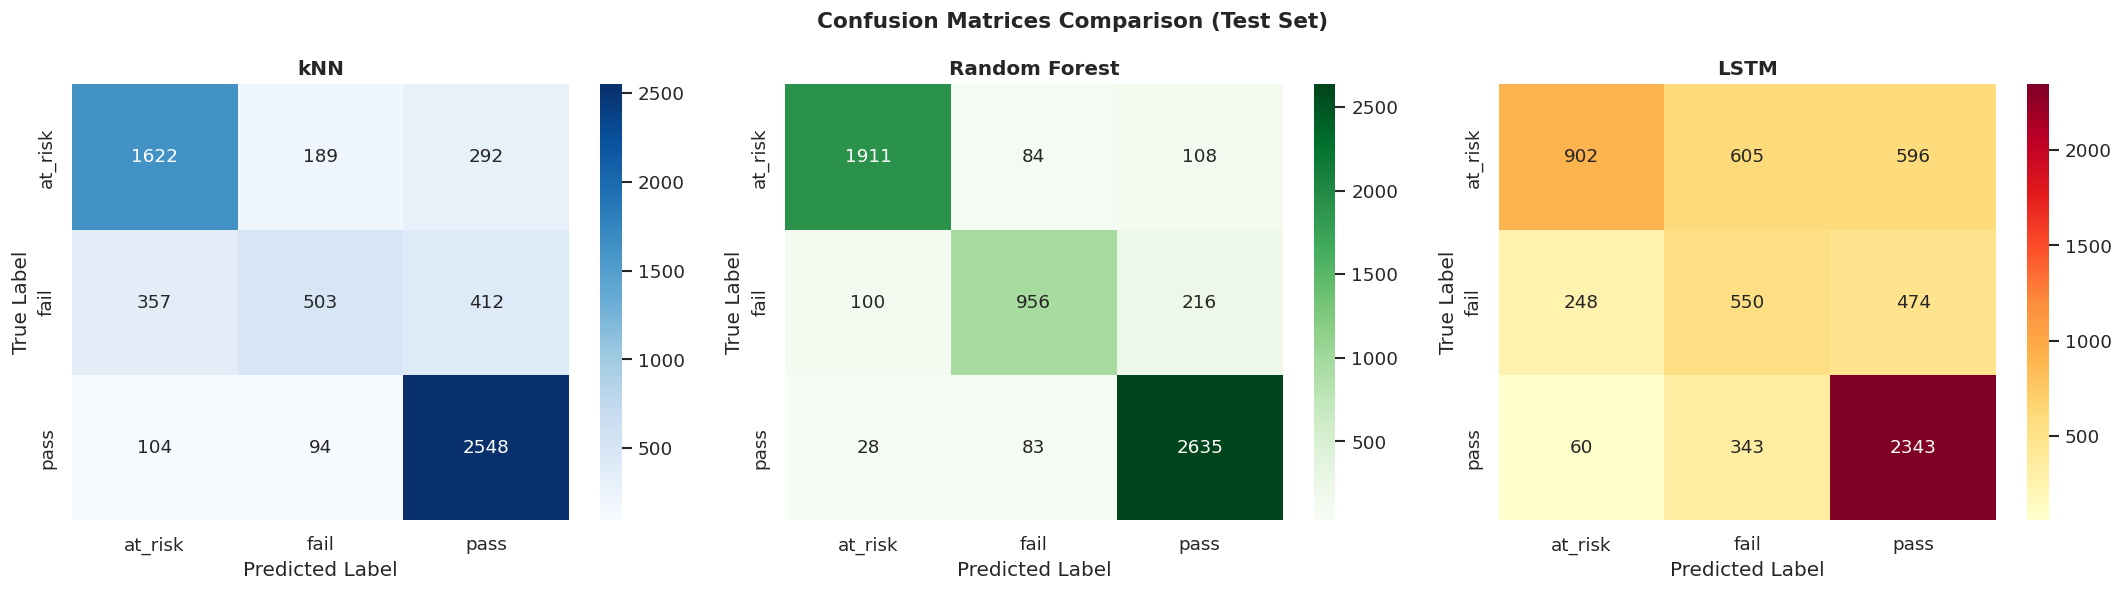
\includegraphics[width=\columnwidth]{figures/results/classification_conf_mat.png}
    \caption{Side-by-side Confusion Matrices for kNN, RF and LSTM}
    \label{fig:classification_conf_mat}
\end{figure}

The Random Forest model additionally yielded interpretable feature importance rankings. The five most important features by Gini impurity were assessment completion rate, composite risk score, missed assessment risks, average assessment score, and tma\_count. Demographic features ranked markedly lower, corroborating findings from \cite{2} and \cite{14} that behavioural signals dominate demographic predictors in educational outcome modelling. The LSTM's temporal architecture conferred a particular advantage in identifying at-risk students whose engagement declined significantly after the first few weeks of study which is a pattern consistent with the early warning signal literature \cite{9}.

\begin{figure}[htbp]
    \centering
    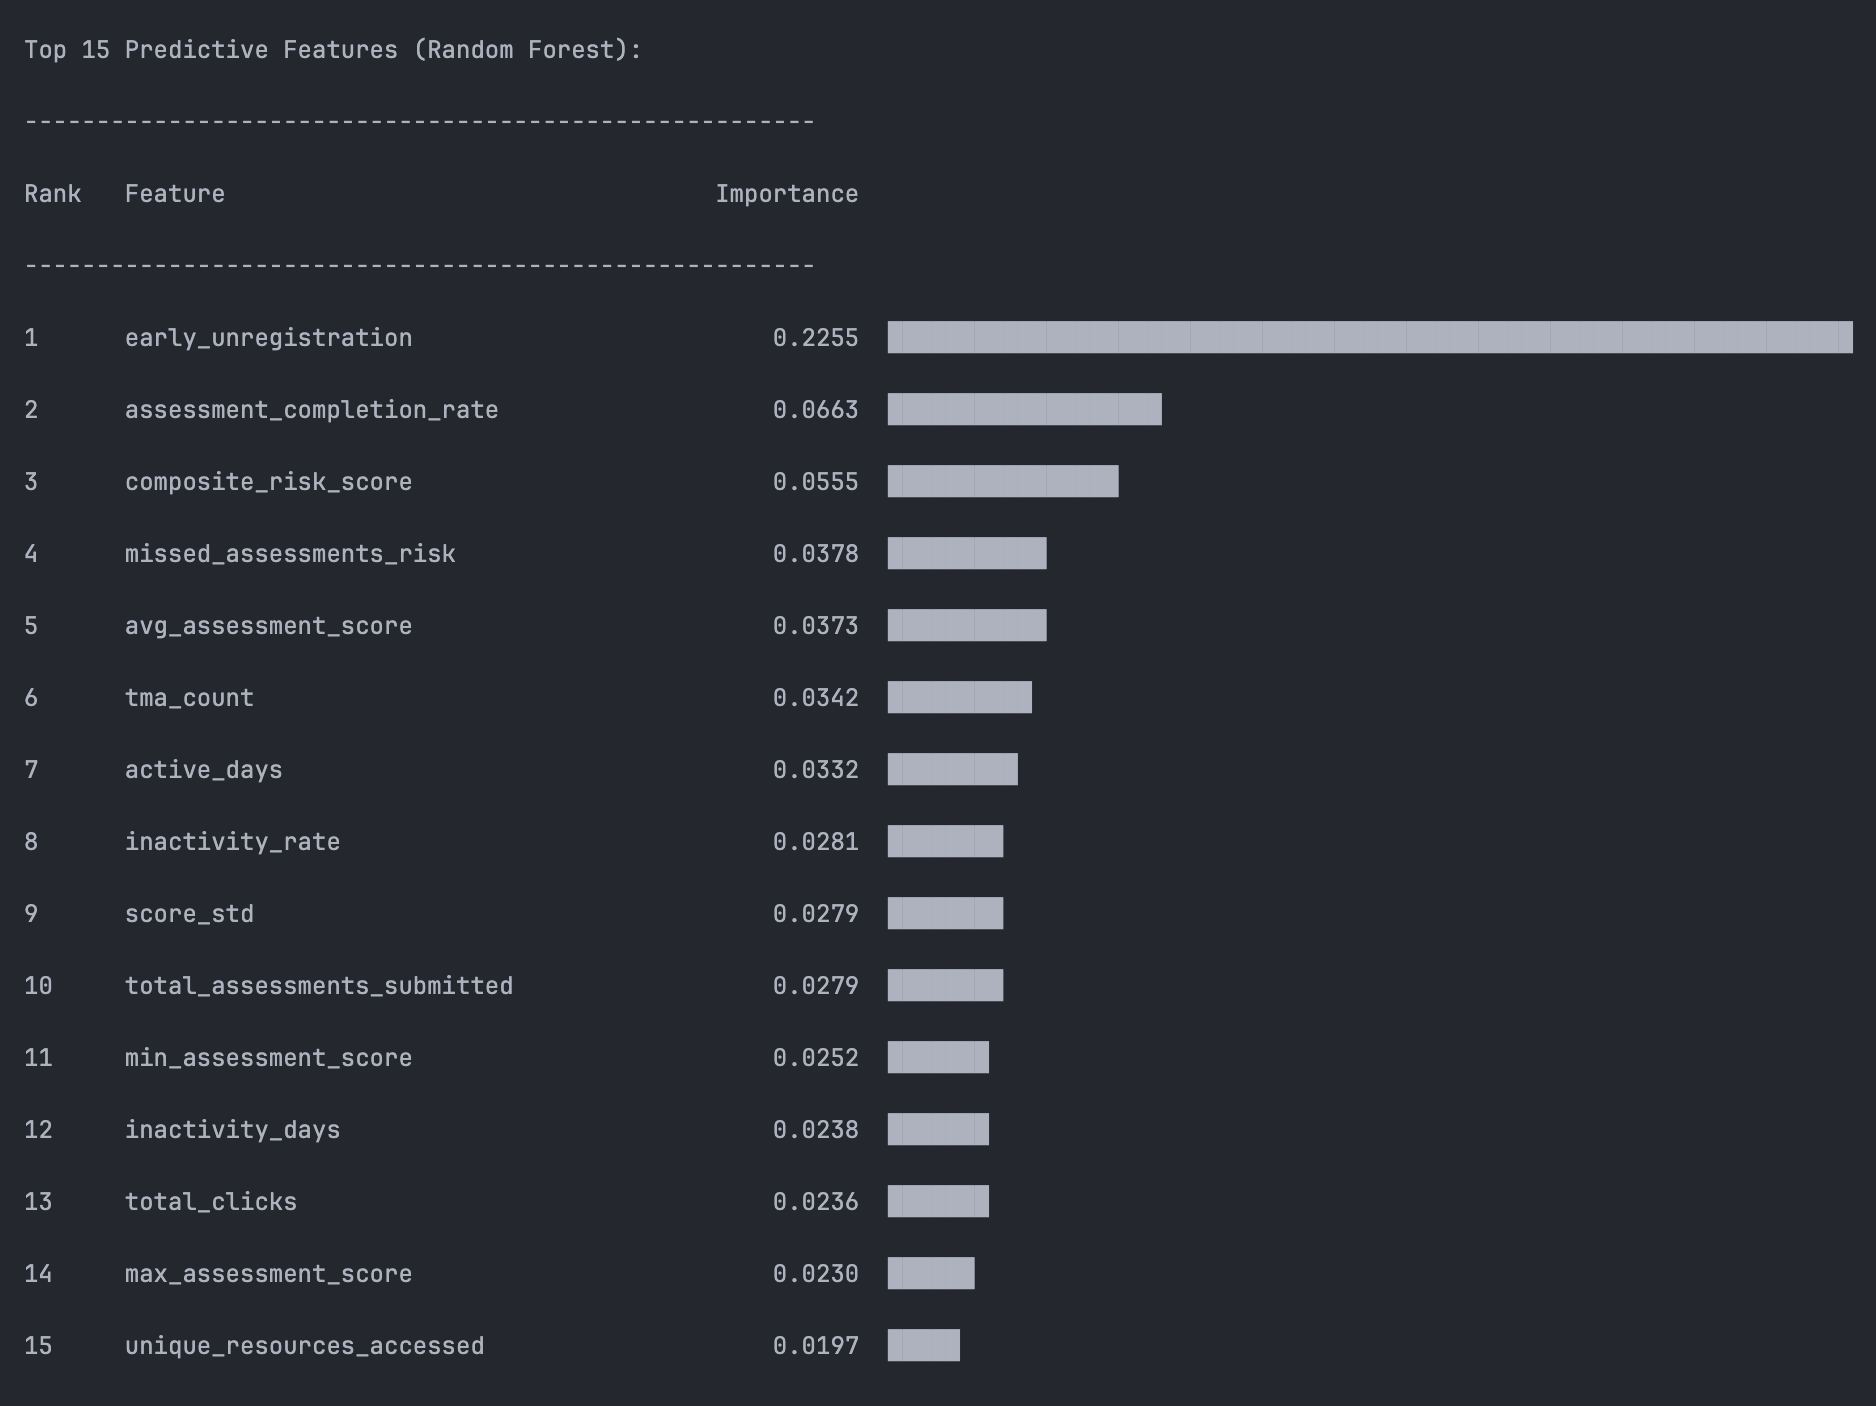
\includegraphics[width=\columnwidth]{figures/results/classification_rf_top_features.png}
    \caption{Top 15 Random Forest features importance}
    \label{fig:classification_rf_top_features}
\end{figure}

\subsubsection{Regression Results}
Table~\ref{tab:reg_results} summarises the test-set regression metrics for the three gradient boosting models. All three models achieved competitive performance, with LightGBM emerging as the top performer by R\textsuperscript{2}, followed closely by CatBoost and XGBoost.

\begin{table}[h!]
\centering
\caption{Regression Model Comparison: Test Set}
\label{tab:reg_results}
\begin{tabular}{lcccc}
\toprule
\textbf{Model} & \textbf{RMSE $\downarrow$} & \textbf{MAE $\downarrow$} & \textbf{MAPE\% $\downarrow$} & \textbf{R\textsuperscript{2} $\uparrow$} \\ \midrule
LightGBM  & 1.133 & 0.700 & 1.217 & 0.9946 \\
CatBoost  & 1.187 & 0.745 & 1.282 & 0.9940 \\
XGBoost   & 1.174 & 0.708 & 1.159 & 0.9942 \\ \bottomrule
\end{tabular}
\end{table}

\begin{figure}[htbp]
    \centering
    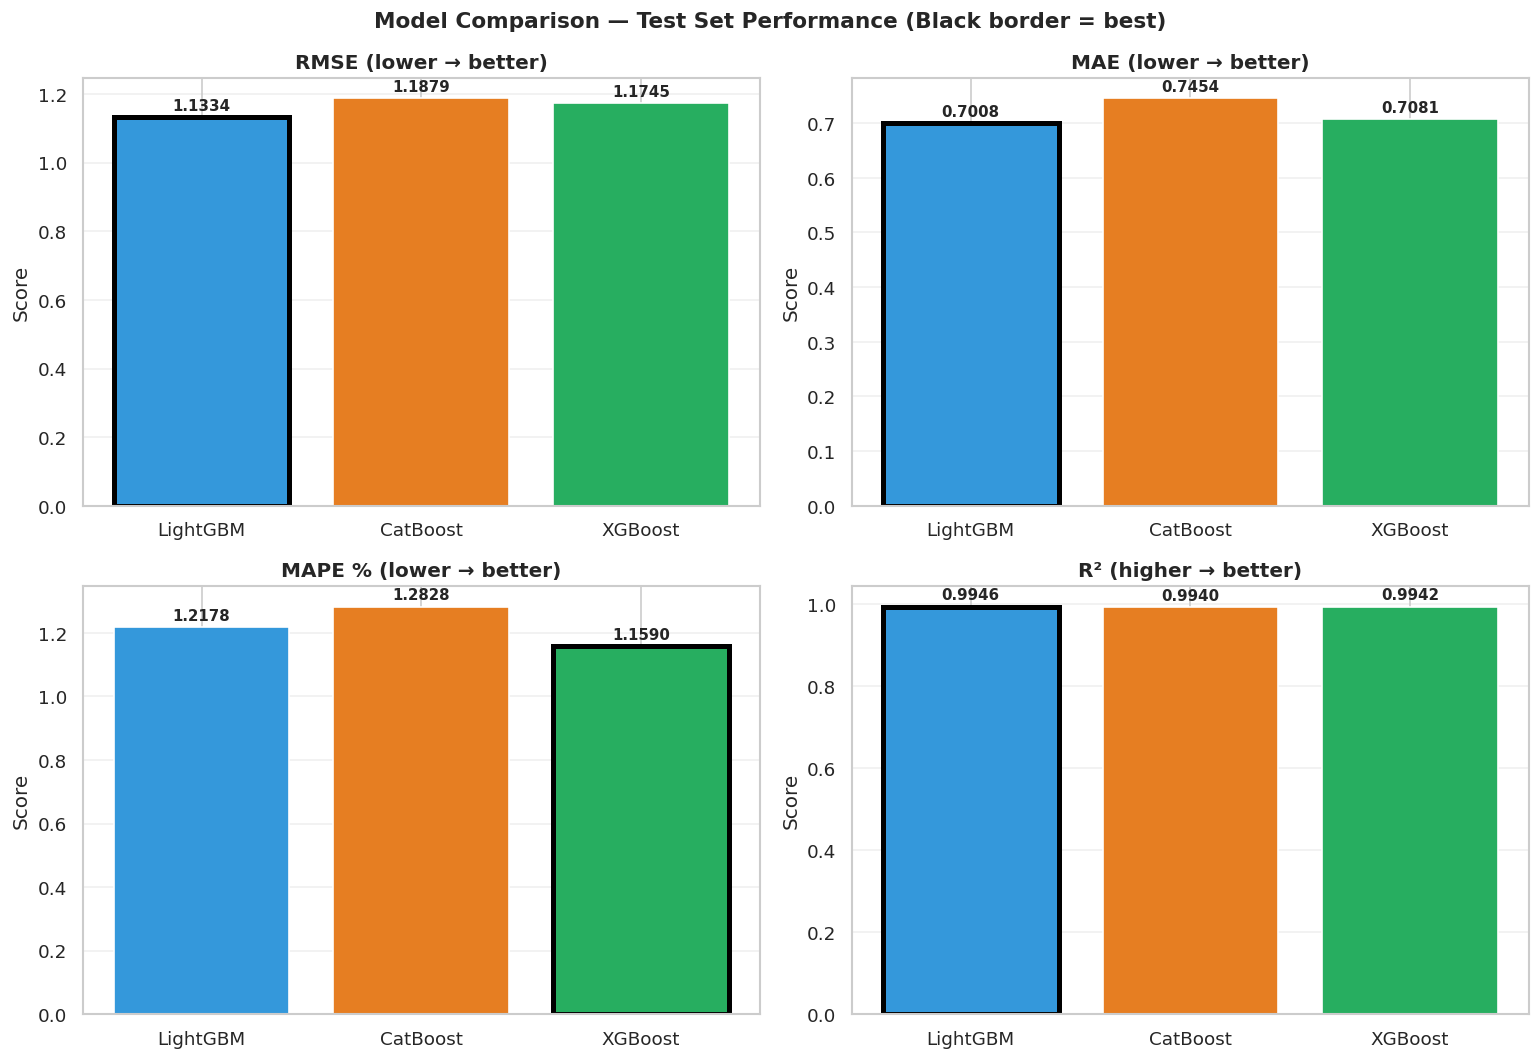
\includegraphics[width=\columnwidth]{figures/results/regression_test_results.png}
    \caption{Bar chart comparing LightGBM, CatBoost, XGBoost on four metrics}
    \label{fig:regression_test_results}
\end{figure}

\subsubsection{Temporal Feature Importance in Regression}
The consensus feature importance analysis across all three regression models revealed that maximum score features contributed the greatest aggregate importance, followed by min score and Phase 6 average assessment score feature. This finding is consistent with the educational literature suggesting that high engagement to obtain high scores is the strongest indicator of final performance \cite{9}. The \textit{asmt\_assessment\_count} feature and total unique resources also ranked among the top predictors, confirming that students with more variety resources and high assessment completion rate do well.

\begin{figure}[htbp]
    \centering
    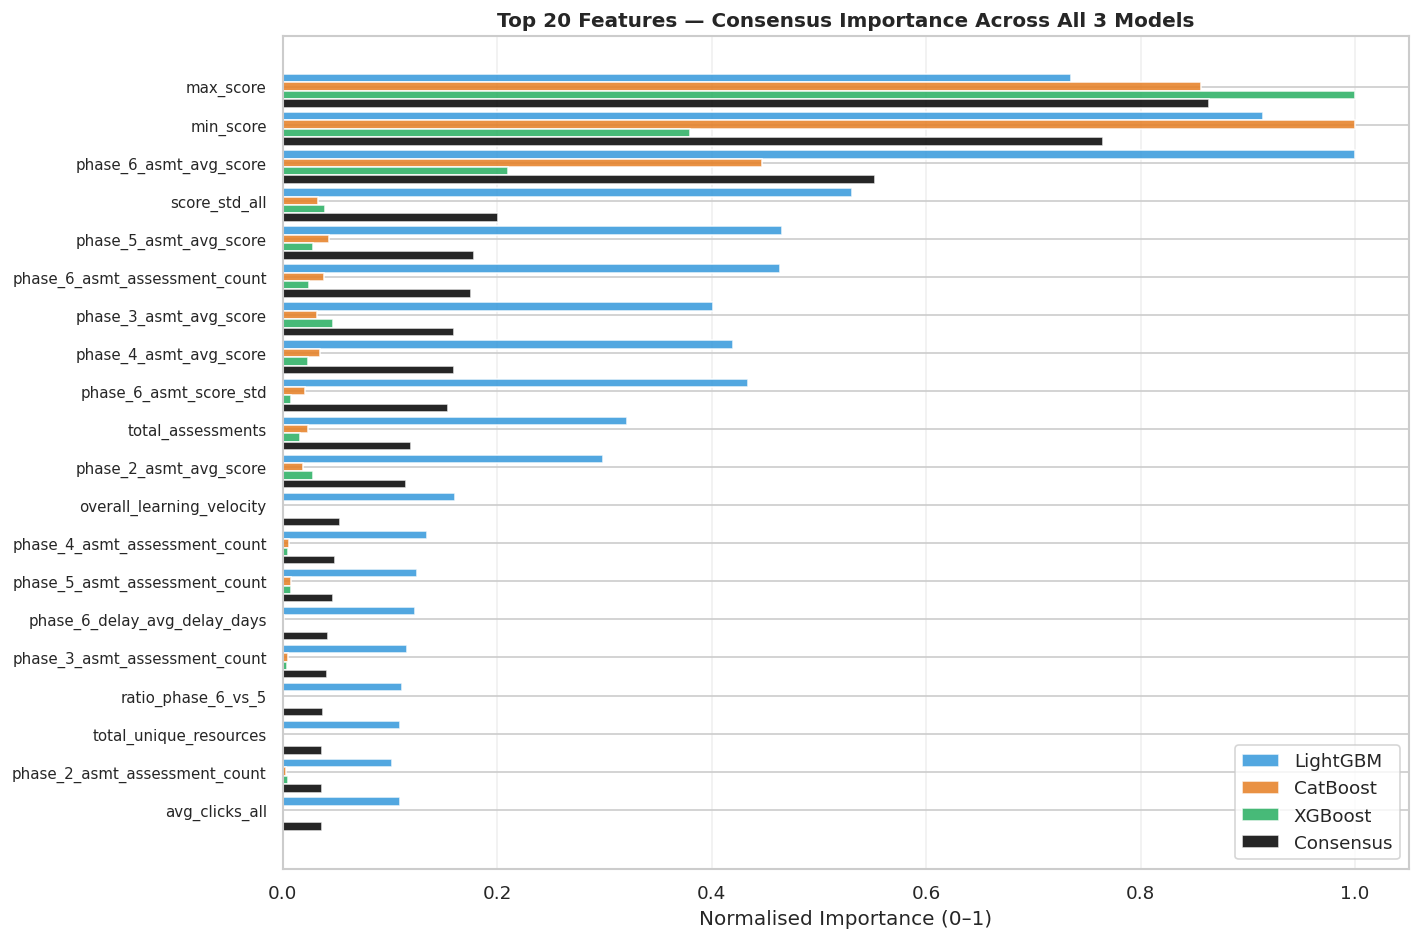
\includegraphics[width=\columnwidth]{figures/results/regression_top_features.png}
    \caption{Top 20 consensus features importance (averaged across all models)}
    \label{fig:regression_top_features}
\end{figure}

\subsubsection{At-Risk Student Profile}
Profiling the at-risk (Withdrawn) student group against successful (pass) students revealed a consistent behavioural signature: at-risk students generated on average fewer total VLE clicks, had fewer active study days, exhibited lower assessment completion rates, and produced higher composite risk scores. The inactivity rate for at-risk students was markedly higher than for passing students, indicating extended periods of zero engagement. Early intervention triggers derived from these patterns include: total clicks below 50 in the first two weeks, zero active days after registration, and a score below 40 on the first assessment.


% =========================================================================== %
\section{Conclusion}
\label{sec:conclusion}

This paper has presented a comprehensive, dual-task machine learning framework for predicting student outcomes in online higher education using the OULAD dataset. Three classification models, kNN, Random Forest, and LSTM  were developed and evaluated for the three-class outcome prediction task (pass, fail, at-risk), while three gradient boosting regressors, LightGBM, CatBoost, and XGBoost were applied to the continuous assessment score prediction task. The entire pipeline was implemented with distributed processing via Apache PySpark to handle millions of VLE clickstream records.

The principal finding is that behavioural engagement features, particularly total VLE clicks, active study days, and temporal phase engagement, are markedly stronger predictors of student outcome than demographic attributes. This result holds across all models and both tasks, and it aligns with and reinforces prior literature on VLE-based prediction \cite{1, 3}. The time-segmented feature engineering approach of partitioning course engagement into six 30-day phases revealed that other than the core assessment related metrics, mid-course disengagement (Phase 3) is the single most predictive behavioural window, providing educators with an actionable intervention target.

The resulting system has the potential to be integrated into any Learning Management System as an early warning pipeline, flagging at-risk students within the first three weeks of a course which is early enough for proactive tutoring contact to be effective. Limitations include the temporal age of the OULAD dataset (collected before the COVID-19 pandemic significantly altered online learning behaviour), its specificity to the Open University UK context, and the absence of social or peer interaction features. Future work should explore transformer-based sequence models, federated learning for cross-institution generalisability, and A/B testing frameworks to empirically evaluate the impact of model-driven interventions on actual retention rates.

% =========================================================================== %
\section*{References}
\begin{thebibliography}{00}

\bibitem{1} M. Jawad, A. Khlaif, S. Farhan, and R. Salim, ``Students' academic performance and engagement prediction in a virtual learning environment using random forest with data balancing,'' \textit{IEEE Access}, vol. 10, pp. 48481--48492, 2022.

\bibitem{2} M. Vermeulen and M. Volman, ``Promoting student engagement in online education: Online learning experiences of Dutch university students,'' \textit{Distance Education}, vol. 45, no. 2, pp. 185--202, 2024.

\bibitem{3} A. Alnassar, F. Alhajlah, and A. Almutairi, ``How well a student performed? A machine learning approach to classify students' performance on virtual learning environment,'' \textit{IEEE Access}, vol. 9, pp. 113828--113843, 2021.

\bibitem{4} Y. Li and J. Xue, ``Dynamic interaction between student learning behaviour and learning environment,'' \textit{Journal of Educational Technology \& Society}, vol. 26, no. 1, pp. 58--71, 2023.

\bibitem{5} C. Akpen, N. Allotey, and O. Osei, ``Impact of online learning on student's performance and engagement: A systematic review,'' \textit{Education and Information Technologies}, vol. 29, no. 4, pp. 4781--4803, 2024.

\bibitem{6} Z. Hussain, A. Hussain, and M. Hussain, ``A flexible feature selection approach for predicting students' academic performance in online courses,'' \textit{Computers \& Education}, vol. 183, p. 104501, 2022.

\bibitem{7} N. Rasheed, A. Khan, and M. Shafi, ``Facilitating flexible learning by replacing classroom time with an online learning environment: A systematic review of blended learning in higher education,'' \textit{Computers \& Education}, vol. 175, p. 104317, 2021.

\bibitem{8} A. Martin and H. Bolliger, ``Student perceptions of online active learning practices and online learning climate predict online course engagement,'' \textit{Online Learning}, vol. 26, no. 1, pp. 1--23, 2022.

\bibitem{9} E. Ntourmas, N. Avouris, and D. Daskalaki, ``Does time matter in analyzing educational data? A new dataset for streaming learning analytics,'' \textit{IEEE Transactions on Learning Technologies}, vol. 16, no. 3, pp. 364--376, 2023.

\bibitem{10} O. Kizilcec, E. Pérez-Sanagustín, and J. Maldonado, ``Persistence and time challenges in an open online university: A case study of the experiences of first-year learners,'' \textit{Computers in Human Behavior}, vol. 146, p. 107801, 2023.

\bibitem{11} A. Bozkurt, N. Akgün-Özbek, and O. Zawacki-Richter, ``The tensions between student dropout and flexibility in learning design: The voices of professors in open online higher education,'' \textit{International Review of Research in Open and Distributed Learning}, vol. 23, no. 2, pp. 1--22, 2022.

\bibitem{12} R. Waheed, A. Kaur, and N. Ain, ``Predictive modelling with the open university learning analytics dataset OULAD: A systematic literature review,'' \textit{Computers \& Education: Artificial Intelligence}, vol. 2, p. 100011, 2021.

\bibitem{13} M. Alqahtani and H. Mohammad, ``Factors influencing online learning satisfaction,'' \textit{European Journal of Educational Research}, vol. 10, no. 3, pp. 1253--1267, 2021.

\bibitem{14} C. Zhang, J. Xu, and L. Wang, ``E-learning behavior categories and influencing factors of STEM courses: A case study of the open university learning analysis dataset (OULAD),'' \textit{Computers \& Education}, vol. 181, p. 104451, 2022.

\bibitem{15} R. Assunção Flores and P. Duarte Silveira, ``An extensive examination of varied approaches in e-learning and MOOC research: A thorough overview,'' \textit{Interactive Learning Environments}, vol. 31, no. 10, pp. 6391--6410, 2023.

\bibitem{16} B. Kardan, A. Bentahar, and N. Benachour, ``Streaming approaches for temporal educational data mining and learning analytics,'' \textit{Expert Systems with Applications}, vol. 202, p. 117275, 2022.

\end{thebibliography}

\end{document}
